\section{Lectura geométrica}
\label{sec:limites:geometrica}
\label{sec:hallazgos:limites-rates}

En el plan Pro de Resend el \textit{rate} es de 10 peticiones por segundo, el valor por defecto que el proveedor publica por equipo, compartido por todas sus claves de API \citep{resenddocs}.
A ese ritmo, un mes de 30 días admite 25.920.000 peticiones, y la cuota del plan es de 50.000 correos al mes \citep{resendpricing}.
Al ritmo máximo, en esos 30 días cabría, por tanto, 518 veces la cuota, contando un destinatario por petición.
En SendGrid Essentials 50K \citep{sendgridpricing} el mismo cálculo da 518.400 veces, con un \textit{rate} de 10.000 peticiones por segundo.
El proveedor publica ese \textit{rate} una sola vez, en una pregunta frecuente que no lo liga a ningún plan.
En la cuenta de prueba de Mailchimp Transactional el cálculo no se puede hacer.
Su franquicia de 500 correos no tiene ventana declarada, y lo único que pone tiempo es un caudal de 25 correos a la hora \citep{mailchimpdocs}.

El cálculo usa cuatro magnitudes de la Datasheet.
El \textit{rate} $R$ se expresa en peticiones por segundo y sale del bloque \texttt{max\_power}.
La cuota $Q$ se expresa en correos, y su ventana $W$, el periodo tras el que la cuota se repone (un día o un mes), en segundos.
Las dos están en el bloque \texttt{capacity}.
El factor $k$ es el número de destinatarios que lleva cada petición, de uno al máximo que admite el proveedor, que la Datasheet declara en el bloque \texttt{workload}.

El factor $k$ corresponde al «CRF» (\textit{Consumption Request Factor}) de Gavira Sánchez \citep{gavira2026tfm}, la regla que dice cuántas unidades de una métrica descuenta cada petición.
Contar $k$ en destinatarios supone que cada destinatario descuenta una unidad de cuota.
Esa equivalencia está sostenida en cuatro de las ocho APIs: Resend y SendGrid la publican, y en Brevo y Amazon SES la midió un sondeo, una tanda de peticiones reales contra la API para medir un límite (Apartado~\ref{sec:propuesta:validacion}).
En Postmark, MailerSend, Mailgun y Mailchimp no consta que cada destinatario descuente una unidad de cuota.

Para un envío uniforme a un ritmo medio $c$, en correos por segundo, los dos límites fijan dos umbrales de ritmo y un tiempo:
\begin{equation}
c_{\mathrm{cuota}} = \frac{Q}{W}, \qquad c_{\mathit{rate}} = R \cdot k, \qquad t_{\min} = \frac{Q}{R \cdot k}.
\label{eq:limites-rates}
\end{equation}
El primer umbral es el ritmo medio que agota la cuota justo al cerrar su ventana.
El segundo es el ritmo máximo de correos que admite el \textit{rate}.
El tiempo $t_{\min}$ es el que tarda una ráfaga sostenida a ese ritmo máximo en agotar la cuota.

De los dos límites, la restricción activa es el de umbral menor: el que se alcanza primero y frena el envío, mientras el otro no llega a actuar.
En Resend Pro la cuota pide 0,019 correos por segundo de media y el \textit{rate} admite 10, así que la restricción activa es la cuota.
El cociente $R \cdot W / Q$ compara los dos topes en la misma ventana: cuántas veces cabría la cuota en lo que el \textit{rate} admite en ella: 518 en Resend Pro y 518.400 en SendGrid Essentials 50K.
Se calcula con $k = 1$ para comparar las APIs en peticiones, y $k$ solo entra en el umbral del \textit{rate} y en $t_{\min}$.

Las cuatro magnitudes son las que PRIME4API lee de la Datasheet para construir los límites de cada plan \citep{gavira2026tfm}.
El mes se toma de 30 días (2.592.000 segundos) y el día de 86.400 segundos.
Con meses de 31 días los cocientes cambian un 3,3~\%.

Con ocho APIs, esta notación no cubre tres casos: los dos contadores de Mailgun, el caudal de Mailchimp en correos por hora y su franquicia sin ventana.
En Mailgun, la cabecera de la respuesta de cada envío aceptado trae dos contadores sobre el mismo \textit{endpoint}: uno de 80.000 peticiones y otro de 2.000.000 de destinatarios.
Los dos comparten una ventana que Mailgun no publica y que dos mediciones situaron en unos diez segundos (Sección~\ref{sec:limites:publicado}).
Hay entonces dos términos de \textit{rate}, $R$ en peticiones y $R_d$ en destinatarios, y cuál de los dos corta antes depende de $k$.
La Tabla~\ref{tab:limites-rates-b} calcula el cociente de Mailgun con el contador de peticiones, y el de destinatarios solo entra en su $t_{\min}$ con el $k$ máximo.

En Mailchimp el caudal se declara en correos por hora y no en peticiones, así que $k$ no multiplica nada: el \textit{rate} solo frena el envío cuando el ritmo medio supera los 25 correos por hora.
La franquicia de 500 correos de su cuenta de prueba tampoco tiene ventana.
Sin $W$ no hay cociente que formar, porque los 500 correos de la franquicia se gastan una sola vez y no se reponen.
En Mailchimp no se calcula el cociente y se anota el tipo de límite.

La misma relación se lee como una curva.
Ruiz-Cortés y Ruiz-López interpretan el \textit{rate} como la velocidad máxima de consumo y la cuota como el volumen máximo acumulable en un periodo, y la capacidad efectiva sale de aplicar los dos límites a la vez \citep{ruizcortes2025cajanegra}.
El ACM adopta esa interpretación como su semántica.
Sobre ella, la curva de capacidad $C(t)$ de Gavira Sánchez \citep{gavira2026tfm} es el máximo de correos acumulables desde el inicio de la ventana hasta el instante $t$ sin violar ningún límite.

Con un \textit{rate} y una cuota, la curva tiene dos tramos.
Mientras manda el \textit{rate}, la curva es una recta de pendiente $R \cdot k$.
Cuando manda la cuota, se vuelve horizontal a la altura de $Q$.
El codo entre ambos cae en $t_{\min}$.
Cuanto antes llega el codo dentro de la ventana, más holgado es el \textit{rate}.
Esa holgura se mide con $W / t_{\min} = R \cdot W \cdot k / Q$, que es el cociente $R \cdot W / Q$ multiplicado por $k$.
En Resend Pro con $k = 1$ el codo llega a los 5.000 segundos, unos 83 minutos, y el tramo horizontal ocupa el resto de los 30 días.
Con los 50 destinatarios por petición que admite Resend, el codo se adelanta a los 100 segundos.
La curva no recoge los dos contadores de Mailgun ni la franquicia sin ventana de Mailchimp.

\begin{figure}[H]
\centering
\subfigure[Resend Pro, $k = 1$ (3 horas)]{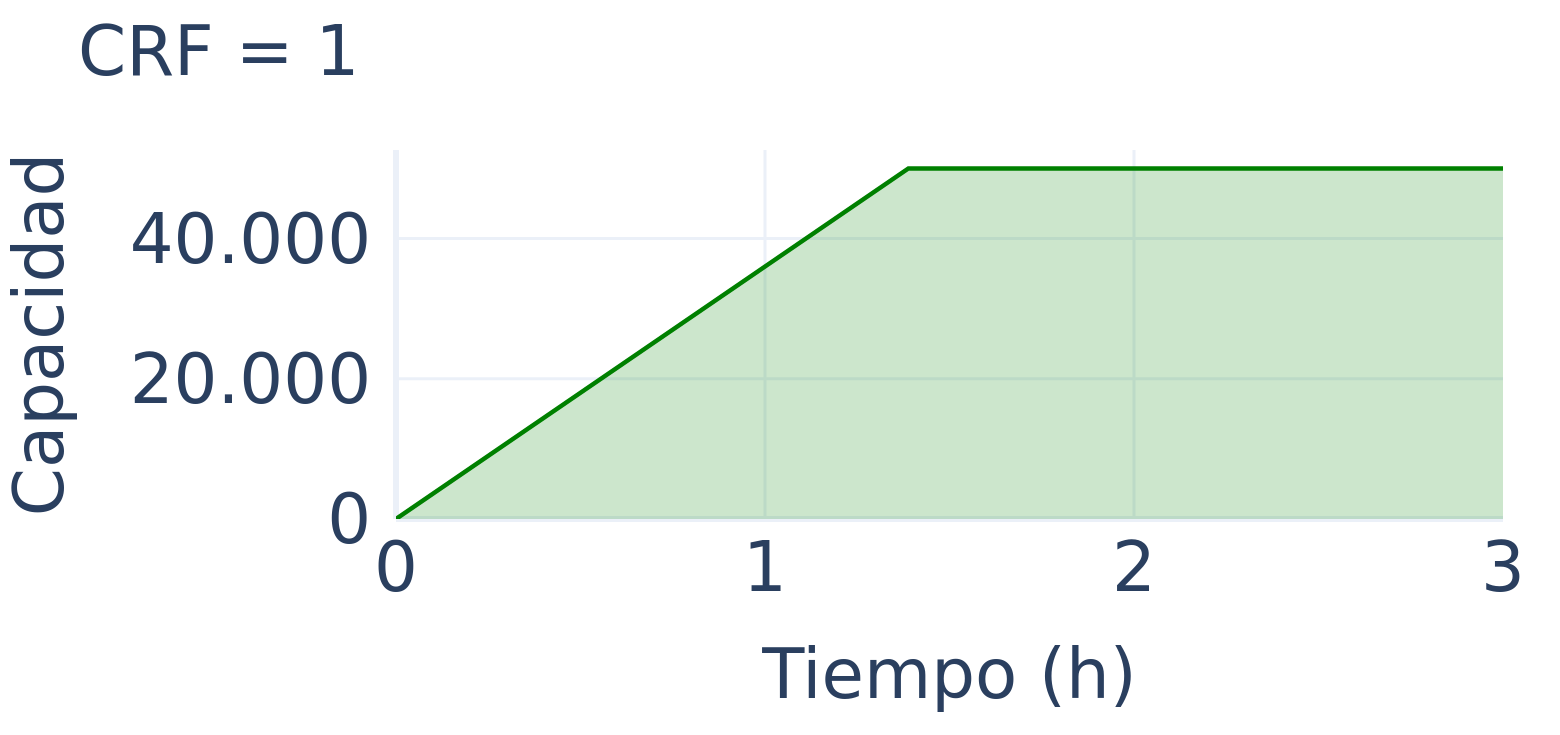
\includegraphics[width=0.42\textwidth]{fig/capacidad_resend_pro_k1_2026-10-25.png}}
\subfigure[SendGrid Essentials 50K, $k = 1.000$ (5 segundos)]{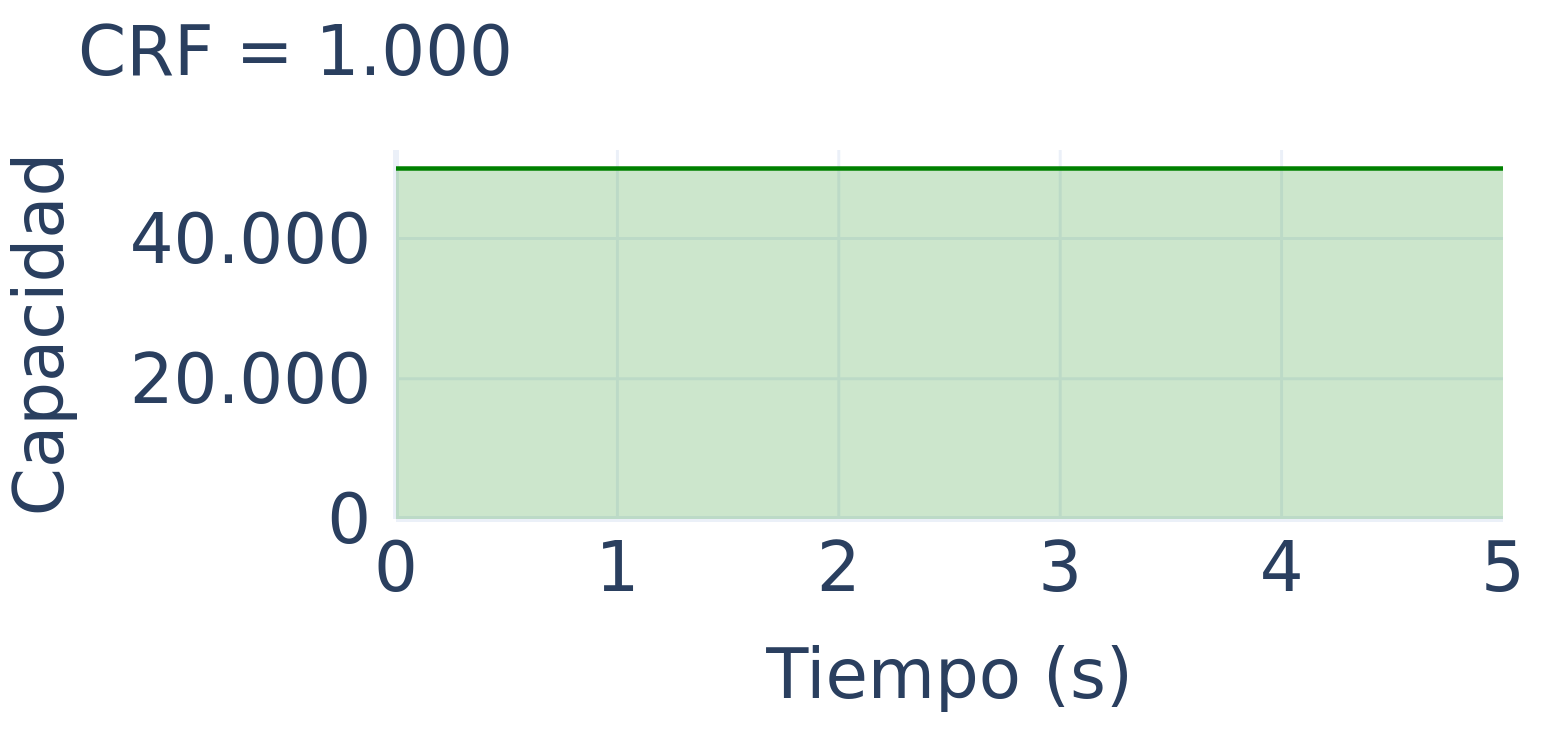
\includegraphics[width=0.42\textwidth]{fig/capacidad_sendgrid_essentials_k1000_2026-10-25.png}}
\subfigure[MailerSend Hobby, $k = 1$ (1 hora)]{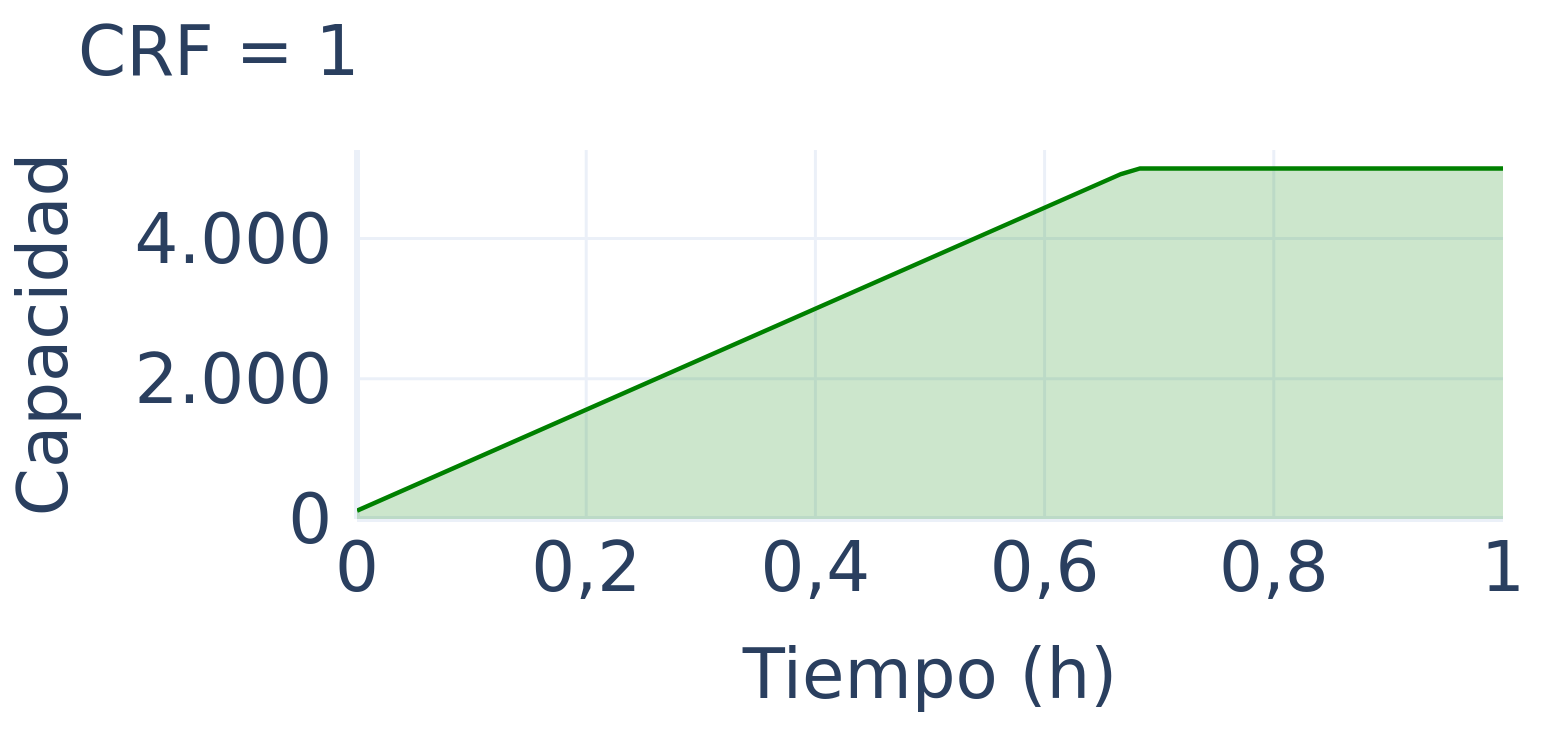
\includegraphics[width=0.42\textwidth]{fig/capacidad_mailersend_hobby_k1_2026-10-25.png}}
\subfigure[Amazon SES, los cuatro planes, $k = 1$ (10 minutos)]{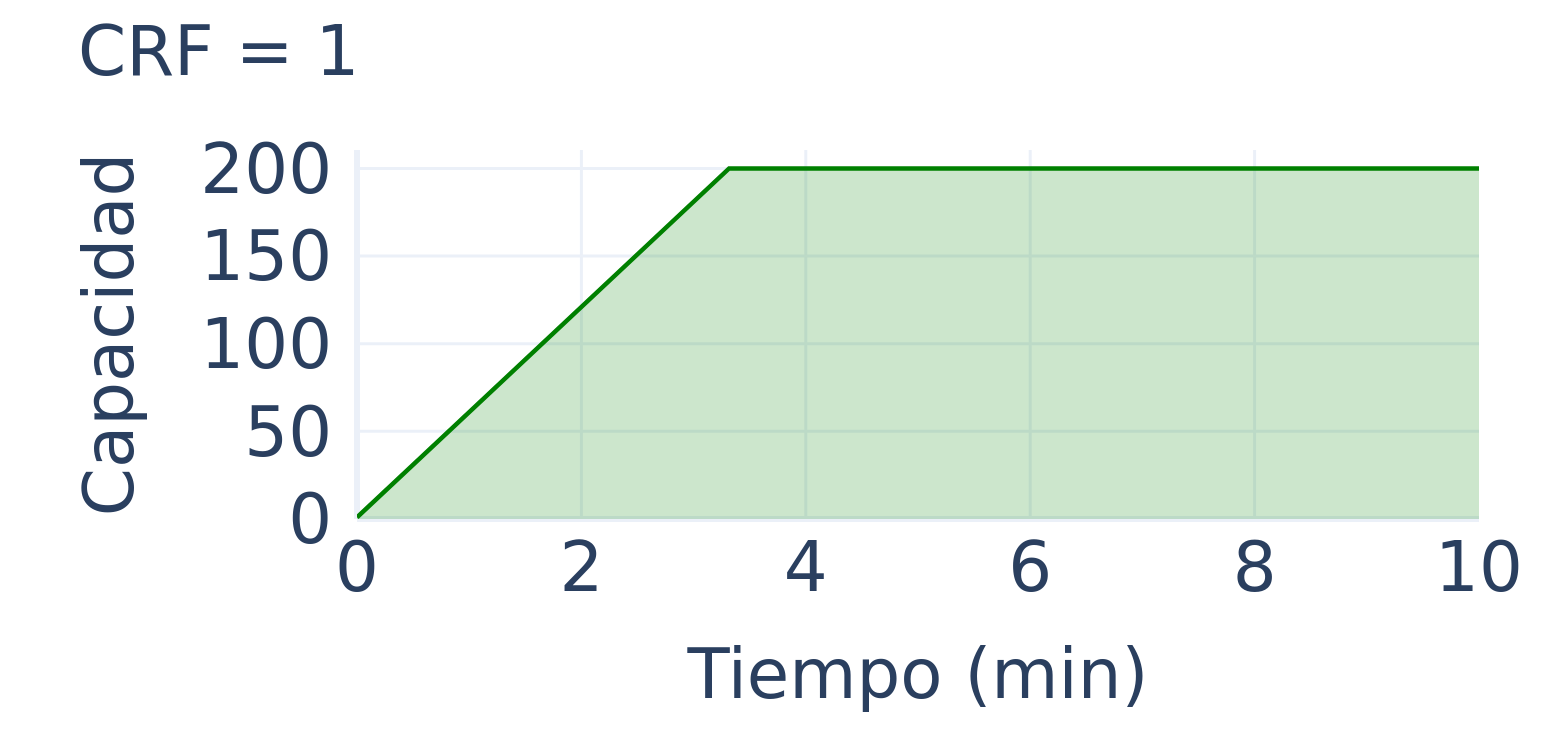
\includegraphics[width=0.42\textwidth]{fig/capacidad_ses_pro_k1_2026-10-25.png}}
\caption[Curva de capacidad $C(t)$ de Resend Pro, SendGrid Essentials 50K, MailerSend Hobby y Amazon SES]{Curva de capacidad $C(t)$ de cuatro planes, dibujada por PRIME4API \citep{prime4apirepo} en local. Entre paréntesis, el intervalo que muestra cada gráfica. Tras el codo, la curva sigue horizontal hasta que la cuota se repone: a los 30 días en Resend, SendGrid y MailerSend, y a las 24 horas en Amazon SES. El área sombreada es la capacidad acumulable.}
\label{fig:capacidad}
\end{figure}

La Figura~\ref{fig:capacidad} muestra la curva de cuatro planes.
La dibuja el propio PRIME4API \citep{prime4apirepo}, ejecutado en local con la misma imagen de contenedor que despliega SPHERE.
El motor lee las Datasheets y su renderizador traza la curva.
Cada gráfica muestra el intervalo que hace visible el codo, porque en una ventana de 30 días el tramo inclinado no se distinguiría de una vertical.
El motor da por enviadas en el instante $t = 0$ las peticiones que el \textit{rate} admite en su primer periodo, un segundo en Resend Pro y un minuto en MailerSend Hobby.
Esa es la primera ráfaga, y por eso el motor da 4.999 segundos en Resend Pro donde el cálculo a mano da 5.000.

En SendGrid Essentials 50K se toma $k = 1.000$, el máximo de destinatarios que el proveedor admite por petición.
Con él la cuota cabe en 50 peticiones, el tramo inclinado dura cinco milésimas de segundo y la curva alcanza la cuota casi desde el origen.
En MailerSend Hobby con $k = 1$ el tramo inclinado sube 120 correos por minuto y el codo llega a los 41 minutos, con una cuota de 5.000 correos al mes.
La gráfica de MailerSend Hobby se pide en correos, la unidad que fija el parámetro \texttt{capacity\_unit} del motor, y por eso no muestra la cuota diaria de peticiones del plan (Apartado~\ref{subsec:evolucion:h1}).
Con esa cuota diaria de 1.000 peticiones, los 5.000 correos con $k = 1$ tardan 4 días y 8 minutos, y no 41 minutos.

En Amazon SES el precio del plan no cambia la curva.
Sus cuatro planes, los tres de la página de precios y la tarifa por uso sin plan, de 0 a 500 USD al mes, devuelven la misma curva, porque la Datasheet les asigna la misma cuota y el mismo caudal.
Son los del entorno de pruebas (\textit{sandbox}), el único para el que Amazon publica cifras.
Toda cuenta nueva de SES empieza en ese entorno, solo puede enviar a direcciones y dominios verificados, y pasa a producción cuando el titular lo pide y Amazon lo aprueba.
En ese entorno el \textit{rate} es de una petición por segundo.
Con un destinatario por petición, la cuota de 200 correos al día se agota en 200 segundos (199 en el motor), y la cuenta no envía nada más hasta que la cuota se repone, a las 24 horas.

El entorno de pruebas es un estado de la cuenta: la condición en que el proveedor tiene la cuenta o su suscripción, con independencia del plan contratado.
El estado de la cuenta reúne el estado de la suscripción, como la cuenta en pruebas o pendiente de aprobación, y la reputación, que separa la cuenta sana de la cuenta en revisión.
En el catálogo, MailerSend baja el \textit{rate} con la cuenta en revisión, y la cuenta de prueba de Mailchimp Transactional tiene su propio caudal de 25 correos por hora.
Una cuenta en estado sano es la que está aprobada y sin restricción por reputación.
El Apartado~\ref{subsec:evolucion:p06} separa el estado de la suscripción de la reputación con el caso de MailerSend.
